% begin module area-between-curves-Horizontal
\begin{frame}
Some regions are best treated by regarding $x$ as a function of $y$. If a region is bounded by curves with equations $ x=f(y) $, and $ x=g(y) $, where $ f $ and $ g $ are continuous and $ f(y)\ge g(y) $ for  $ c\le y \le  d $ (see Figure), then its area is
\[
A=\int_c^d f(y)-g(y)dy
\]
If we write $ x_R $ for the right boundary and $ x_L $ for the left boundary, then $ \ds A=\int_c^d(x_R-x_L)dy $\\
%\column{.65\textwidth}


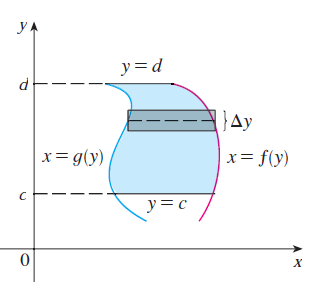
\includegraphics[width=0.4\linewidth]{../../modules/area-between-curves/pictures/H1.PNG}\;\;\;
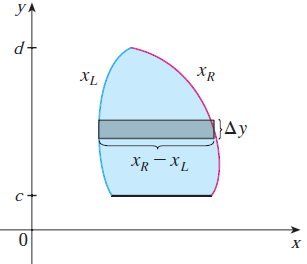
\includegraphics[width=0.4\linewidth]{../../modules/area-between-curves/pictures/H2.PNG}\\




\end{frame}


\begin{frame}
\begin{example}%[Example 6, p. 426]
Find the area enclosed by the line $ y=x-1 $ and the parabola $ y^2=2x-6$\\
Solution: \pause 
\begin{columns}
\column{.4\textwidth}
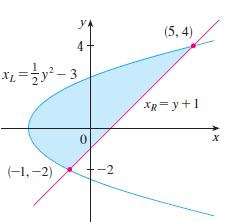
\includegraphics[width=0.8\linewidth]{../../modules/area-between-curves/pictures/H3.PNG}\\
\column{.65\textwidth}
By solving the two equations for $ x $ we find that the points of intersection, $(-1,-2)$ and $(5,4)$ and we get 
\[  x_L= \frac{y^2}{2}-3, \textrm{ and }  x_R=y+1. \]
\uncover<2->{
So we get $\ds  A=\int_{-2}^4(x_R-x_L)\;dy$ } 
 \end{columns}
 \vspace*{-3mm}
 \begin{align*}
 \uncover<3->{A= \int_{-2}^4 (y+1) -(\frac{y^2}{2}-3)\;dy}&\uncover<4->{= \int_{-2}^4 -\frac{y^2}{2}+y+4\;dy}\\  
 \uncover<5->{&=\left.-\frac{y^3}{6}+\frac{y^2}{2}+4y\right|_{-2}^4}\\ 
 \uncover<6->{&=(-\frac{64}{6}+8+16)-(-\frac{4}{3}+2-8)=18}
 \end{align*}
\end{example}
\end{frame}
% end module area-between-curves-ex5


\begin{frame}
\textbf{NOTE:} We could have found the area in the last example by integrating with respect to $ x $ instead of $ y $, but the calculation is much more involved. It would have meant splitting the region in two and computing the areas labeled $ A_1 $ and $ A_2 $ and in diagram below. The method we used is \textit{much} easier.\\
\begin{center}
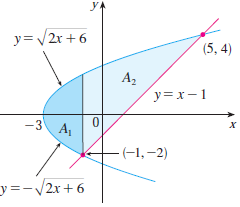
\includegraphics[width=0.5\linewidth]{../../modules/area-between-curves/pictures/H4.PNG}
\end{center}

\end{frame}